\chapter{द्वि-घटकी ठोस--द्रव आरेख}\label{ch:b2:solid-liquid-diagrams}

टिन \qty{232}{\degreeCelsius} पर पिघलता है और सीसा \qty{327}{\degreeCelsius} पर,
फिर भी बिजली-मिस्त्रियों का पुराना सोल्डर, जो इन दोनों का मिश्रण है,
\qty{182}{\degreeCelsius} पर, दोनों से नीचे, पिघलता है। सड़क पर बिखेरा गया नमक बर्फ़ पिघलाता है, परंतु केवल
लगभग \qty{-21}{\degreeCelsius} तक; अधिक ठंडी रात में वह कुछ नहीं करता।
दूसरी ओर, ताँबा और निकेल ठोस में भी किसी भी अनुपात में मिल जाते हैं, और उनकी
मिश्रधातुएँ दोनों धातुओं के गलनांकों के बीच तापों के एक परिसर में पिघलती हैं।
इस अध्याय के आरेख हर युग्म के लिए बताते हैं कि ठंडे होते द्रव से कौन-से ठोस
क्रिस्टलित होते हैं, किन तापों पर और कितनी
मात्राओं में --- यही ज्ञान हर ढलाई, हर सोल्डर जोड़ और हर
निम्न-गलनांकी मिश्रधातु के पीछे है।

\begin{recall}
\Cref{ch:b2:chemical-potential}: \omterm{def:b2:chemical-potential:ideal-mixture}{आदर्श मिश्रण} में किसी घटक का \omterm{def:b2:chemical-potential:chemical-potential}{रासायनिक विभव},
हिमांकमिति। \Cref{ch:b2:equilibrium-shifts}: \omterm{def:b2:equilibrium-shifts:variance}{स्वातंत्र्य कोटि}।
\Cref{ch:b2:liquid-vapour-diagrams}: \omterm{def:b2:liquid-vapour-diagrams:binary-diagram}{द्वि-घटकी आरेख}, संयोजी रेखाएँ और \omterm{thm:b2:liquid-vapour-diagrams:lever}{उत्तोलक
नियम}। प्रथम वर्ष का खंड: धात्विक आबंधन, प्रतिस्थापनी और अंतराकाशी
मिश्रधातुएँ, क्रिस्टल के प्रकार।
\end{recall}

\begin{omfigure}
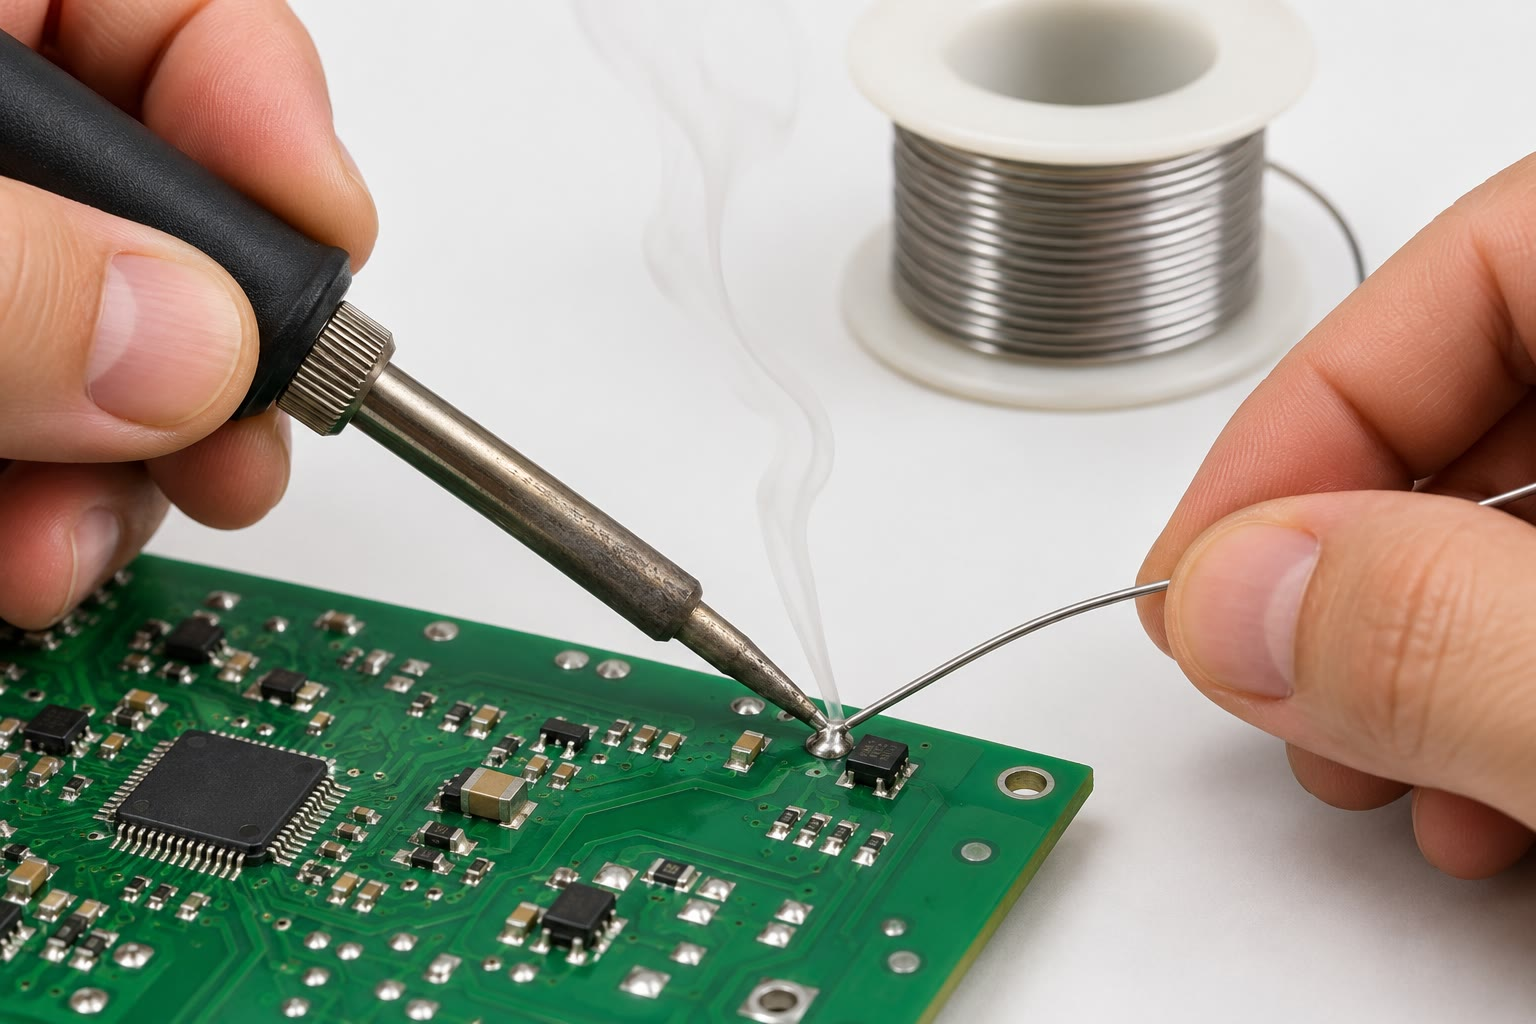
\includegraphics[width=0.6\linewidth]{images/book3/ai/b2-08-soldering.jpg}

{\small सर्किट बोर्ड पर किसी घटक की सोल्डरिंग: सोल्डर का तार गर्म आयरन के
संपर्क में आते ही पिघलता है और आयरन हटाते ही एक सेकंड के भीतर जोड़ जम जाता है
--- क्योंकि मिश्रधातु एक ही, निम्न ताप पर पिघलती है।}
\end{omfigure}

\section{ऊष्मीय विश्लेषण}

\begin{definition}[ऊष्मीय विश्लेषण]\label{def:b2:solid-liquid-diagrams:cooling-curve}
\emph{ऊष्मीय विश्लेषण}\index{ऊष्मीय विश्लेषण} किसी नमूने के अवस्था-परिवर्तनों के
ताप उसके उस ताप से निर्धारित करता है जो उसे स्थिर दर से गर्म या ठंडा
करते समय दर्ज किया जाता है। धीमे शीतलन के दौरान समय के सापेक्ष ताप का अभिलेख
\emph{शीतलन वक्र}\index{शीतलन वक्र} कहलाता है।
\end{definition}

किसी भी अवस्था-परिवर्तन से दूर नमूना सुचारु रूप से ठंडा होता है। जब कोई ठोस
क्रिस्टलित होना आरंभ करता है, तो क्रिस्टलन की ऊष्मा शीतलन को धीमा कर देती है: वक्र
प्रवणता में एक मोड़ दिखाता है, या कुछ समय के लिए स्थिर ताप पर रुक जाता है --- एक
\textit{पठार} --- यदि हिमीकरण नियत ताप पर होता है।

\begin{proposition}[पठार]\label{prop:b2:solid-liquid-diagrams:plateaus}
नियत दाब पर शुद्ध पदार्थ स्थिर ताप पर जमता है, और
वह द्वि-घटकी द्रव भी जिससे दो ठोस साथ-साथ क्रिस्टलित होते हैं। जिस द्वि-घटकी
द्रव से एक ठोस क्रिस्टलित होता है, वह तापों के एक परिसर में जमता है।
\end{proposition}

\begin{proof}
दाब नियत होने पर \omterm{def:b2:equilibrium-shifts:variance}{स्वातंत्र्य कोटि} $v = n - r + 1 - \varphi$ है। शुद्ध
पदार्थ, द्रव + ठोस: $v = 1 + 1 - 2 = 0$। द्वि-घटकी, द्रव + दो ठोस:
$v = 2 + 1 - 3 = 0$। द्वि-घटकी, द्रव + एक ठोस: $v = 2 + 1 - 2 = 1$: ताप
द्रव के संघटन के साथ बदलता है। \omterm{def:b2:equilibrium-shifts:variance}{स्वातंत्र्य कोटि} 0 का अर्थ है कि जब तक सभी प्रावस्थाएँ
उपस्थित हैं, ताप नहीं बदल सकता: हटाई गई ऊष्मा हिमीकरण से आती है,
जब तक कोई प्रावस्था लुप्त न हो जाए।
\end{proof}

\begin{omfigure}
\begin{tikzpicture}[font=\small, x=0.55cm, y=0.05cm]
  \foreach \dx/\name in {0/शुद्ध धातु, 9/{मिश्रण, पहले एक ठोस}, 18/गलनक्रांतिक मिश्रण} {
    \draw[->] (\dx,0) -- (\dx+7.5,0) node[below left, font=\scriptsize] {$t$};
    \draw[->] (\dx,0) -- (\dx,62) node[above, font=\scriptsize] {$T$};
    \node[font=\scriptsize] at (\dx+3.8,-8) {\name};
  }
  % pure: cool, plateau at 40, cool
  \draw[omDef, thick] (0,58) .. controls (1,48) and (1.6,42) .. (2,40) -- (4.5,40) .. controls (5.2,32) and (6,24) .. (7,20);
  \node[font=\scriptsize, anchor=south] at (3.25,40.5) {पठार};
  % mixture: cool, break at 48, slow fall, plateau at 30, cool
  \draw[omDef, thick] (9,58) .. controls (9.6,53) and (9.9,50) .. (10.2,48)
     .. controls (11,42) and (11.6,35) .. (12.3,30) -- (14.2,30) .. controls (14.9,23) and (15.6,17) .. (16.5,14);
  \node[font=\scriptsize, anchor=west] at (10.4,49.5) {मोड़};
  \node[font=\scriptsize, anchor=south] at (13.25,30.5) {गलनक्रांतिक};
  % eutectic: plateau at 30
  \draw[omDef, thick] (18,58) .. controls (19,46) and (19.8,36) .. (20.5,30) -- (24,30) .. controls (24.7,23) and (25.4,17) .. (26.2,14);
  \node[font=\scriptsize, anchor=south] at (22.25,30.5) {पठार};
\end{tikzpicture}

{\small \omterm{def:b2:solid-liquid-diagrams:cooling-curve}{शीतलन वक्र}, व्यवस्था-रूप। शुद्ध धातु पठार पर जमती है। मिश्रण
पहले ठोस के प्रकट होने पर प्रवणता में मोड़ दिखाता है, फिर तापों के एक परिसर में
जमने वाले द्रव का धीमा शीतलन, फिर गलनक्रांतिक का
पठार। गलनक्रांतिक संघटन वाला द्रव शुद्ध पदार्थ की तरह एक ही पठार पर
जमता है।}
\end{omfigure}

\begin{method}[शीतलन वक्रों से आरेख बनाना]\label{met:b2:solid-liquid-diagrams:diagram-from-curves}
\begin{enumerate}
  \item शुद्ध घटकों सहित संघटनों की एक श्रृंखला के लिए \omterm{def:b2:solid-liquid-diagrams:cooling-curve}{शीतलन वक्र}
        दर्ज कीजिए।
  \item (संघटन, ताप) आलेख पर हर संघटन के लिए पहले मोड़ (क्रिस्टलन का
        आरंभ) का और हर पठार का ताप
        अंकित कीजिए।
  \item पहले क्रिस्टलन के बिंदुओं को जोड़िए: यही \omterm{def:b2:solid-liquid-diagrams:liquidus}{लिक्विडस} है। हिमीकरण के
        अंतिम बिंदुओं को जोड़िए: \omterm{def:b2:solid-liquid-diagrams:liquidus}{सॉलिडस}। अनेक संघटनों के लिए समान ताप पर मिलने वाला
        पठार एक अपरिवर्ती रेखा (गलनक्रांतिक) है।
  \item गलनक्रांतिक पठार की लंबाई, जो गलनक्रांतिक संघटन पर
        सबसे अधिक होती है, उस संघटन की स्थिति बताती है।
\end{enumerate}
\end{method}

\section{ठोस में पूर्ण मिश्रणीयता}

\begin{definition}[ठोस विलयन]\label{def:b2:solid-liquid-diagrams:solid-solution}
\emph{ठोस विलयन}\index{ठोस विलयन} परिवर्ती संघटन वाली एक अकेली क्रिस्टलीय प्रावस्था
है, जिसमें एक घटक के परमाणु उसी जालक के स्थलों पर दूसरे घटक के परमाणुओं का
स्थान लेते हैं (प्रतिस्थापनी) या उस जालक के रिक्त स्थानों में बैठते हैं
(अंतराकाशी)।
\end{definition}

ताँबे और निकेल की फलक-केंद्रित घनीय संरचना एक ही है और उनके परमाणुओं की
त्रिज्याएँ निकट हैं: वे हर संघटन पर प्रतिस्थापनी \omterm{def:b2:solid-liquid-diagrams:solid-solution}{ठोस विलयन} बनाते हैं।

\begin{definition}[लिक्विडस और सॉलिडस]\label{def:b2:solid-liquid-diagrams:liquidus}
ठोस--द्रव आरेख पर \emph{लिक्विडस}\index{लिक्विडस} वह वक्र है
जिसके ऊपर सब कुछ द्रव है; यह किसी ठोस के साथ साम्य में द्रव का संघटन
देता है। \emph{सॉलिडस}\index{सॉलिडस} वह वक्र है जिसके नीचे
सब कुछ ठोस है; जहाँ ठोस एक विलयन है, वहाँ यह द्रव के साथ साम्य में ठोस का
संघटन देता है।
\end{definition}

\begin{proposition}[लेंस]\label{prop:b2:solid-liquid-diagrams:lens}
यदि दोनों घटक द्रव में और ठोस में आदर्श विलयन बनाते हैं, तो
\omterm{def:b2:solid-liquid-diagrams:liquidus}{लिक्विडस} और \omterm{def:b2:solid-liquid-diagrams:liquidus}{सॉलिडस} दोनों गलनांकों को जोड़ते हैं और एक
लेंस-आकार द्वि-प्रावस्थी क्षेत्र घेरते हैं; हर ताप पर द्रव और ठोस में हर
घटक के मोल अंश $x_i$ इस प्रकार संबंधित हैं:
\[
  \frac{x_i^{\ell}}{x_i^{s}} = \exp\left[-\frac{\Delta_{\text{गलन}}H_i}{R}\left(\frac1T - \frac1{T_i^*}\right)\right] .
\]
\end{proposition}

\begin{proof}\emergencystretch=3em
$i$ का \omterm{def:b2:chemical-potential:chemical-potential}{रासायनिक विभव} दोनों प्रावस्थाओं में समान है, $\mu_i^{*,s} +
RT\ln x_i^s = \mu_i^{*,\ell} + RT\ln x_i^\ell$, अतः $RT\ln(x_i^\ell/x_i^s) =
-(\mu_i^{*,\ell} - \mu_i^{*,s}) = -\Delta_{\text{गलन}}G_i(T)$, और स्थिर
$\Delta_{\text{गलन}}H_i$ के साथ $\Delta_{\text{गलन}}G_i = \Delta_{\text{गलन}}H_i(1 - T/T_i^*)$।
हर प्रावस्था में $x_1 + x_2 = 1$ के साथ ये दोनों संबंध हर $T$ पर दोनों
संघटन नियत करते हैं (चित्र के लिए संख्यात्मक रूप से हल किए गए); परिणामी
वक्रों का लेंस बनाना स्वीकार किया गया है।
\end{proof}

\begin{omfigure}
\begin{tikzpicture}
\begin{axis}[omphase, width=0.62\linewidth, height=7cm, ymin=1050, ymax=1480,
  xlabel={$x$ (निकेल)}, ylabel={$T$ (\unit{\degreeCelsius})}]
\addplot[omliquidus] table[x=xl, y=T] {figdata/out/bachelor-2-solid-liquid-a.dat};
\addplot[omsolidus] table[x=xs, y=T] {figdata/out/bachelor-2-solid-liquid-a.dat};
\draw[tieline] (axis cs:0.541,1300) -- (axis cs:0.609,1300);
\fill (axis cs:0.58,1300) circle (1.3pt);
\node[font=\scriptsize] at (axis cs:0.25,1400) {द्रव};
\node[font=\scriptsize] at (axis cs:0.8,1150) {ठोस विलयन};
\node[font=\scriptsize, anchor=east] at (axis cs:0.5,1330) {लिक्विडस};
\node[font=\scriptsize, anchor=west] at (axis cs:0.66,1290) {सॉलिडस};
\node[font=\scriptsize, anchor=west] at (axis cs:0.03,1080) {\qty{1085}{\degreeCelsius}};
\draw[black!50] (axis cs:0.005,1084) -- (axis cs:0.03,1080);
\node[font=\scriptsize, anchor=south east] at (axis cs:1.0,1456) {\qty{1455}{\degreeCelsius}};
\end{axis}
\end{tikzpicture}

{\small ताँबा--निकेल, दोनों धातुओं के गलनांकों और गलन एन्थैल्पियों से आदर्श ठोस
और द्रव विलयनों के लिए परिकलित।
\qty{1300}{\degreeCelsius} पर संघटन 0.58 वाली मिश्रधातु 0.541 के द्रव
और 0.609 के ठोस में बँट जाती है (खंडित संयोजी रेखा)।}
% ledger: tfus:Cu, dfus:Cu, tfus:Ni, dfus:Ni
\end{omfigure}

\begin{method}[ठोस--द्रव आरेख पढ़ना]\label{met:b2:solid-liquid-diagrams:read-solid-liquid}
\begin{enumerate}
  \item द्रव से आरंभ करके समग्र संघटन की ऊर्ध्वाधर रेखा का नीचे की ओर
        अनुसरण कीजिए।
  \item \omterm{def:b2:solid-liquid-diagrams:liquidus}{लिक्विडस} पर पहला ठोस प्रकट होता है; उसका संघटन संयोजी रेखा के
        दूसरे सिरे (\omterm{def:b2:solid-liquid-diagrams:liquidus}{सॉलिडस}, या कोई शुद्ध घटक) पर पढ़ा जाता है।
  \item द्वि-प्रावस्थी क्षेत्र में संयोजी रेखा के सिरों पर दोनों संघटन
        और \omterm{thm:b2:liquid-vapour-diagrams:lever}{उत्तोलक नियम} से अनुपात पढ़िए, मोल अंशों के साथ मोल में,
        द्रव्यमान अंशों के साथ द्रव्यमान में।
  \item किसी क्षैतिज अपरिवर्ती रेखा पर ताप तब तक रुका रहता है जब तक कोई प्रावस्था
        समाप्त न हो जाए; उसके नीचे प्रावस्थाओं का नया युग्म पढ़िए।
\end{enumerate}
\end{method}

\begin{example}[\qty{1300}{\degreeCelsius} पर एक मिश्रधातु]\label{ex:b2:solid-liquid-diagrams:lever}
\qty{1300}{\degreeCelsius} पर निकेल मोल अंश 0.58 वाली मिश्रधातु के लिए
ठोस में परमाणुओं का अंश $(0.58 - 0.541)/(0.609 - 0.541) = 0.57$ है।
लगभग \qty{1315}{\degreeCelsius} पर प्रकट होने वाला पहला ठोस मिश्रधातु से निकेल में
अधिक समृद्ध है, अंतिम द्रव उससे निर्धन।
\end{example}

आरेख साम्य का वर्णन करता है, जो ठोस में धीमा होता है: निकेल से समृद्ध पहले क्रिस्टल,
द्रव के बदलने के साथ उसमें उत्तरोत्तर निर्धन परतों से ढक जाते हैं,
और ठोस में विसरण को उन्हें एकसमान करने का समय नहीं मिलता। जल्दी ठंडी की गई
ढलाई \textit{स्तरित} क्रिस्टलों से बनी होती है, जो केंद्र से किनारे तक क्रमिक
रूप से बदलते हैं; \omterm{def:b2:solid-liquid-diagrams:liquidus}{सॉलिडस} से नीचे देर तक गर्म करना उन्हें समांगी बना देता है।

\section{ठोस में कोई मिश्रणीयता नहीं: गलनक्रांतिक}

जब दोनों ठोस बिल्कुल नहीं मिलते, तो हर घटक शुद्ध रूप में क्रिस्टलित होता है, और
\omterm{def:b2:solid-liquid-diagrams:liquidus}{लिक्विडस} की दो शाखाएँ होती हैं, हर ठोस के लिए एक।

\begin{theorem}[श्रोडर--वान लार]\label{thm:b2:solid-liquid-diagrams:schroder}
यदि कोई घटक A आदर्श द्रव मिश्रण से शुद्ध रूप में क्रिस्टलित होता है, तो वह \omterm{def:b2:solid-liquid-diagrams:liquidus}{लिक्विडस}
जिस पर ठोस A प्रकट होता है, यह है:
\[
  \ln x_A = -\frac{\Delta_{\text{गलन}}H_A}{R}\Big(\frac1T - \frac1{T_A^*}\Big),
\]
जहाँ $x_A$ द्रव में A का मोल अंश है, $T_A^*$ और
$\Delta_{\text{गलन}}H_A$ शुद्ध A का गलनांक और गलन एन्थैल्पी
(स्थिर मानी गई)।
\end{theorem}

\begin{proof}
साम्य पर शुद्ध ठोस A का \omterm{def:b2:chemical-potential:chemical-potential}{रासायनिक विभव} द्रव में A के \omterm{def:b2:chemical-potential:chemical-potential}{रासायनिक विभव} के बराबर होता है:
$\mu_A^{*,s}(T) = \mu_A^{*,\ell}(T) + RT\ln x_A$। अतः $R\ln x_A =
-\Delta_{\text{गलन}}G_A(T)/T$। गिब्स--हेल्महोल्ट्ज़ से $d(\Delta_{\text{गलन}}G_A/T)/
dT = -\Delta_{\text{गलन}}H_A/T^2$; $T_A^*$ से, जहाँ
$\Delta_{\text{गलन}}G_A = 0$, $T$ तक समाकलन करने पर $\Delta_{\text{गलन}}G_A/T =
\Delta_{\text{गलन}}H_A(1/T - 1/T_A^*)$ मिलता है।
\end{proof}

तनु विलयन के लिए $\ln x_A = \ln(1 - x_B) \approx -x_B$ और $1/T -
1/T_A^* \approx -\Delta T/T_A^{*2}$: $\Delta T = RT_A^{*2}x_B/\Delta_{\text{गलन}}H_A$,
जो \cref{ch:b2:chemical-potential} का हिमांकमितीय नियम है। बेन्ज़ीन ($T^* =
\qty{278.64}{K}$, $\Delta_{\text{गलन}}H = \qty{9.87}{kJ/mol}$, $M =
\qty{78.11}{g/mol}$) के लिए \omterm{def:b2:chemical-potential:colligative}{हिमांकमितीय स्थिरांक} $RT^{*2}M/\Delta_{\text{गलन}}H$
\qty{5.11}{K.kg/mol} आता है।
% ledger: tfus:benzene, dfus:benzene

\begin{definition}[गलनक्रांतिक]\label{def:b2:solid-liquid-diagrams:eutectic}
किसी द्वि-घटकी निकाय का \emph{गलनक्रांतिक बिंदु}\index{गलनक्रांतिक बिंदु} वह
बिंदु है जहाँ द्रव एक साथ दो ठोसों के साथ साम्य में होता है; यह आरेख के उस भाग में वह
निम्नतम ताप है जिस पर कोई द्रव अस्तित्व में रहता है।
गलनक्रांतिक संघटन वाला द्रव, और दोनों ठोसों का वह महीन घनिष्ठ मिश्रण
जिसमें वह जमता है, \emph{गलनक्रांतिक
मिश्रण}\index{गलनक्रांतिक मिश्रण} कहलाते हैं।
\end{definition}

\begin{corollary}[गलनक्रांतिक वहाँ है जहाँ लिक्विडस की शाखाएँ मिलती हैं]\label{cor:b2:solid-liquid-diagrams:eutectic}
ठोस में अमिश्रणीय और द्रव में आदर्श दो घटकों के लिए
गलनक्रांतिक ताप $T_E$ और संघटन
$x_A(T_E) + x_B(T_E) = 1$ के हल हैं, जहाँ हर $x$ अपने ही ठोस के
श्रोडर--वान लार समीकरण से दिया गया है।
\end{corollary}

\begin{proof}
गलनक्रांतिक पर द्रव दोनों ठोसों से संतृप्त होता है: वह एक साथ दोनों
शाखाओं पर होता है, A में और B में पढ़े गए एक ही संघटन के साथ।
\end{proof}

\begin{omfigure}
\begin{tikzpicture}
\begin{axis}[omphase, width=0.62\linewidth, height=6.5cm, ymin=-25, ymax=85,
  xlabel={$x$ (नैफ़्थलीन)}, ylabel={$T$ (\unit{\degreeCelsius})}]
\addplot[omliquidus] table[x=x, y=T] {figdata/out/bachelor-2-solid-liquid-b-benzene.dat};
\addplot[omliquidus] table[x=x, y=T] {figdata/out/bachelor-2-solid-liquid-b-naphthalene.dat};
\draw[thick] (axis cs:0,-3.55) -- (axis cs:1,-3.55);
\fill (axis cs:0.133,-3.55) circle (1.5pt);
\node[font=\scriptsize, anchor=north] at (axis cs:0.133,-4.5) {E};
\node[font=\scriptsize] at (axis cs:0.45,72) {द्रव};
\node[font=\scriptsize, align=center] at (axis cs:0.65,22) {द्रव + ठोस\\ नैफ़्थलीन};
\node[font=\scriptsize, anchor=south west] at (axis cs:0.08,45) {द्रव + ठोस बेन्ज़ीन};
\draw[thin] (axis cs:0.12,45) -- (axis cs:0.06,0.8);
\node[font=\scriptsize] at (axis cs:0.55,-15) {ठोस बेन्ज़ीन + ठोस नैफ़्थलीन};
\end{axis}
\end{tikzpicture}

{\small बेन्ज़ीन--नैफ़्थलीन, हर ठोस के लिए श्रोडर--वान लार
समीकरण से परिकलित। दोनों शाखाएँ गलनक्रांतिक E पर मिलती हैं,
\qty{-3.5}{\degreeCelsius} और 0.13 नैफ़्थलीन, जिसके नीचे सब कुछ ठोस है।}
% ledger: tfus:benzene, dfus:benzene, tfus:naphthalene, dfus:naphthalene
\end{omfigure}

\begin{example}[बेन्ज़ीन--नैफ़्थलीन मिश्रण का शीतलन]\label{ex:b2:solid-liquid-diagrams:naphthalene}
नैफ़्थलीन मोल अंश 0.5 वाला द्रव \omterm{def:b2:solid-liquid-diagrams:liquidus}{लिक्विडस} की नैफ़्थलीन शाखा तक ठंडा होता है,
लगभग \qty{46}{\degreeCelsius} पर, जहाँ शुद्ध ठोस नैफ़्थलीन
क्रिस्टलित होना आरंभ करती है। द्रव, नैफ़्थलीन खोते हुए, शाखा पर नीचे
फिसलता है; \qty{-3.5}{\degreeCelsius} पर वह गलनक्रांतिक तक पहुँचता है, और शेष
स्थिर ताप पर \omterm{def:b2:solid-liquid-diagrams:eutectic}{गलनक्रांतिक मिश्रण} में जम जाता है। \omterm{thm:b2:liquid-vapour-diagrams:lever}{उत्तोलक नियम} से,
गलनक्रांतिक से ठीक ऊपर, ठोस नैफ़्थलीन मोलों का $(0.5 - 0.133)/(1 - 0.133) =
42~\%$ है, गलनक्रांतिक द्रव 58~\%।
\end{example}

\begin{proposition}[गलनक्रांतिक पठार की लंबाई]\label{prop:b2:solid-liquid-diagrams:plateau-length}
समान द्रव्यमान के नमूनों के लिए, जिन्हें ऊष्मा-निष्कासन की समान दर से ठंडा किया जाए,
गलनक्रांतिक पठार की अवधि गलनक्रांतिक तक पहुँचने वाले द्रव की मात्रा के
समानुपाती होती है, जो गलनक्रांतिक संघटन के लिए अधिकतम और शुद्ध घटकों के लिए
शून्य है।
\end{proposition}

\begin{proof}
पठार पर ताप स्थिर रहता है: हटाई गई ऊष्मा, $\Phi\,\Delta t$, स्थिर दर $\Phi$ पर,
गलनक्रांतिक द्रव के हिमीकरण से मुक्त ऊष्मा, $m_E\,\Delta_{\text{गलन}}h_E$, है। अतः $\Delta t = m_E\,\Delta_{\text{गलन}}h_E/
\Phi$, जो गलनक्रांतिक द्रव के द्रव्यमान $m_E$ के समानुपाती है, जिसे \omterm{thm:b2:liquid-vapour-diagrams:lever}{उत्तोलक
नियम} देता है।
\end{proof}

\section{आंशिक मिश्रणीयता और निश्चित यौगिक}

धातुओं के अधिकांश युग्म ठोस में न पूर्णतः मिश्रणीय होते हैं, न पूर्णतः अमिश्रणीय:
हर एक दूसरे को थोड़ा घोलता है। सीसा द्रव्यमान के अनुसार 19~\% तक टिन घोलता है,
टिन 3.4~\% तक सीसा। तब आरेख में दो \omterm{def:b2:solid-liquid-diagrams:solid-solution}{ठोस
विलयन}, (Pb) और (Sn), और उनके बीच एक गलनक्रांतिक होता है; गलनक्रांतिक रेखा अब
आरेख के किनारों तक नहीं पहुँचती, बल्कि \omterm{def:b2:solid-liquid-diagrams:solid-solution}{ठोस विलयनों} की सीमाओं पर
रुक जाती है।

\begin{omfigure}
\begin{tikzpicture}[font=\small, x=0.075cm, y=0.022cm]
  \draw[->] (0,0) -- (106,0) node[right] {\% Sn (द्रव्यमान)};
  \draw[->] (0,0) -- (0,360) node[above] {$T$ (\unit{\degreeCelsius})};
  \foreach \t in {100,200,300} \draw (0,\t) -- (-1.5,\t) node[left, font=\scriptsize] {\t};
  \foreach \w in {0,20,40,60,80,100} \draw (\w,0) -- (\w,-5) node[below, font=\scriptsize] {\w};
  % invariant points (NIST): Pb 327.5, Sn 231.9, eutectic 182.2 at 62.13; limits 18.91 and 96.59
  \draw[omliquidus] (0,327.5) .. controls (25,290) and (45,235) .. (62.13,182.2);
  \draw[omliquidus] (100,231.9) .. controls (85,215) and (72,200) .. (62.13,182.2);
  \draw[omsolidus] (0,327.5) .. controls (8,280) and (14,220) .. (18.91,182.2);
  \draw[omsolidus] (100,231.9) .. controls (98.5,215) and (97.5,200) .. (96.59,182.2);
  \draw[thick] (18.91,182.2) -- (96.59,182.2);
  \draw[omsolidus, densely dashed] (18.91,182.2) .. controls (12,120) and (6,60) .. (3,20);
  \draw[omsolidus, densely dashed] (96.59,182.2) .. controls (98.5,120) and (99.3,60) .. (99.6,20);
  \fill (62.13,182.2) circle (1.5pt);
  \fill (18.91,182.2) circle (1.2pt); \fill (96.59,182.2) circle (1.2pt);
  \node[anchor=south, font=\scriptsize] at (62.13,186) {E};
  \node[font=\scriptsize] at (55,300) {द्रव};
  \node[font=\scriptsize] at (6,150) {(Pb)};
  \node[font=\scriptsize] at (103,140) {(Sn)};
  \node[font=\scriptsize] at (28,235) {L + (Pb)};
  \node[font=\scriptsize] at (84,192) {L + (Sn)};
  \node[font=\scriptsize] at (55,100) {(Pb) + (Sn)};
  % cooling path at 40 %
  \draw[->, omProp, thick] (40,340) -- (40,30);
  \node[font=\scriptsize, omProp, anchor=south] at (40,342) {40~\%};
  \node[font=\scriptsize, anchor=north east] at (16.6,179) {18.9};
  \node[font=\scriptsize, anchor=north] at (62.13,178) {62.1};
  \node[font=\scriptsize, anchor=north east] at (95.8,178) {96.6};
  \node[font=\scriptsize, anchor=west] at (101,182.2) {\qty{182.2}{\degreeCelsius}};
\end{tikzpicture}

{\small सीसा--टिन आरेख, उसके अपरिवर्ती बिंदुओं से होकर खींचा गया: सीसे
(\qty{327.5}{\degreeCelsius}) और टिन (\qty{231.9}{\degreeCelsius}) के गलनांक,
\qty{182.2}{\degreeCelsius} और 62.1~\% टिन पर गलनक्रांतिक E, गलनक्रांतिक ताप पर \omterm{def:b2:solid-liquid-diagrams:solid-solution}{ठोस
विलयनों} की सीमाएँ (18.9~\% और 96.6~\% टिन)। इन बिंदुओं के बीच के वक्र,
और गलनक्रांतिक से नीचे खंडित विलेयता सीमाएँ,
व्यवस्था-रूप में खींची गई हैं। तीर: 40~\% वाले सोल्डर का शीतलन।}
% ledger: eut:Pb-Sn.T, eut:Pb-Sn.wL, eut:Pb-Sn.wPb, eut:Pb-Sn.wSn, tfus:Pb, tfus:Sn
\end{omfigure}

40~\% टिन वाला सोल्डर \omterm{def:b2:solid-liquid-diagrams:liquidus}{लिक्विडस} पर सीसा-समृद्ध विलयन (Pb) के क्रिस्टल
जमा करते हुए जमना आरंभ करता है; द्रव टिन में समृद्ध होता जाता है, जब तक कि
\qty{182.2}{\degreeCelsius} पर वह गलनक्रांतिक संघटन तक नहीं पहुँचता और प्राथमिक
क्रिस्टलों के चारों ओर (Pb) और (Sn) पटलिकाओं के महीन मिश्रण में जम जाता है।

\begin{omfigure}
\begin{tikzpicture}[font=\small]
  \begin{scope}
    \clip (0,0) circle (2.2);
    \fill[gray!20] (-2.3,-2.3) rectangle (2.3,2.3);
    \foreach \k in {-24,...,24} \draw[gray!65, line width=1.1pt] (-2.4+0.2*\k,-2.4) -- ++(55:6);
    \foreach \cx/\cy/\r/\a in {-0.9/0.8/0.55/10, 0.7/1.0/0.45/40, 0.2/-0.6/0.6/-20, -1.1/-0.9/0.4/70, 1.3/-0.3/0.35/5} {
      \fill[omDef!35, draw=omDef, rotate around={\a:(\cx,\cy)}] (\cx,\cy) ellipse ({\r} and {0.7*\r});
    }
  \end{scope}
  \draw[thick] (0,0) circle (2.2);
  \draw[<-, omProp, thick] (0.7,1.0) -- (3.0,1.6) node[right, text=black] {प्राथमिक (Pb) क्रिस्टल};
  \draw[<-, omProp, thick] (1.6,0.9) -- (3.0,0.5) node[right, text=black, align=left] {गलनक्रांतिक: (Pb) और (Sn)\\ की एकांतर पटलिकाएँ};
\end{tikzpicture}

{\small धीमे शीतलन के बाद 40~\% टिन वाले सोल्डर की सूक्ष्मसंरचना, व्यवस्था-रूप:
(Pb) के प्राथमिक क्रिस्टल, जो \omterm{def:b2:solid-liquid-diagrams:liquidus}{लिक्विडस} और गलनक्रांतिक के बीच बने, दोनों \omterm{def:b2:solid-liquid-diagrams:solid-solution}{ठोस
विलयनों} की पतली एकांतर पट्टिकाओं से बने गलनक्रांतिक के
आधात्री में।}
\end{omfigure}

\begin{definition}[निश्चित यौगिक]\label{def:b2:solid-liquid-diagrams:defined-compound}
\emph{निश्चित यौगिक}\index{निश्चित यौगिक} दोनों घटकों द्वारा बना नियत
संघटन $\mathrm{A}_a\mathrm{B}_b$ वाला ठोस है। उसका
\emph{सर्वांगसम गलन}\index{सर्वांगसम गलन} होता है जब वह अपने ही संघटन वाले
द्रव में पिघलता है: तब \omterm{def:b2:solid-liquid-diagrams:liquidus}{लिक्विडस} का उस संघटन पर एक अधिकतम होता है।
\end{definition}

\omterm{def:b2:solid-liquid-diagrams:defined-compound}{सर्वांगसम गलन} वाला यौगिक आरेख को दो भागों में बाँट देता है: हर आधा, A के साथ
$\mathrm{A}_a\mathrm{B}_b$ और $\mathrm{A}_a\mathrm{B}_b$ के साथ B, अपने आप में
एक आरेख है, अपने गलनक्रांतिक के साथ। अधिकतम का संघटन, मोल
अंश में पढ़ा गया, यौगिक का सूत्र देता है।

\begin{omfigure}
\begin{tikzpicture}[font=\small, x=6cm, y=0.05cm]
  \draw[->] (0,0) -- (1.06,0) node[right] {$x_{\mathrm B}$};
  \draw[->] (0,0) -- (0,95) node[above] {$T$};
  \node[below, font=\scriptsize] at (0,0) {A}; \node[below, font=\scriptsize] at (1,0) {B};
  \node[below, font=\scriptsize] at (0.667,0) {$\tfrac23$};
  \draw[omliquidus] (0,70) .. controls (0.12,58) and (0.25,45) .. (0.35,35);
  \draw[omliquidus] (0.35,35) .. controls (0.45,62) and (0.58,79) .. (0.667,80);
  \draw[omliquidus] (0.667,80) .. controls (0.75,79) and (0.8,68) .. (0.85,50);
  \draw[omliquidus] (0.85,50) .. controls (0.9,56) and (0.95,62) .. (1,65);
  \draw[thick] (0,35) -- (0.667,35); \draw[thick] (0.667,50) -- (1,50);
  \draw[thick] (0.667,0) -- (0.667,80);
  \fill (0.35,35) circle[radius=1.5pt]; \fill (0.85,50) circle[radius=1.5pt];
  \fill (0.667,80) circle[radius=1.5pt];
  \node[anchor=north, font=\scriptsize] at (0.35,34) {E$_1$};
  \node[anchor=north, font=\scriptsize] at (0.85,49) {E$_2$};
  \node[anchor=south, font=\scriptsize] at (0.667,81) {$\mathrm{AB_2}$ पिघलता है};
  \node[font=\scriptsize] at (0.35,80) {द्रव};
  \node[font=\scriptsize, align=center] at (0.33,15) {A +\\ $\mathrm{AB_2}$};
  \node[font=\scriptsize, align=center] at (0.84,25) {$\mathrm{AB_2}$\\ + B};
\end{tikzpicture}

{\small \omterm{def:b2:solid-liquid-diagrams:defined-compound}{निश्चित यौगिक} $\mathrm{AB_2}$ (ऊर्ध्वाधर
रेखा $x_{\mathrm B} = 2/3$ पर) वाला व्यवस्था-रूप आरेख, जो \omterm{def:b2:solid-liquid-diagrams:liquidus}{लिक्विडस} के
अधिकतम पर सर्वांगसम रूप से पिघलता है। आरेख अगल-बगल रखे दो सरल गलनक्रांतिक आरेख है,
गलनक्रांतिकों E$_1$ और E$_2$ के साथ।}
\end{omfigure}

\section{उपयोग}

\paragraph{सोल्डर और निम्न-गलनांकी मिश्रधातुएँ।} सोल्डर को जोड़े जाने वाले भागों
से नीचे पिघलना और बिना लेईदार परिसर के जल्दी जमना चाहिए: गलनक्रांतिक संघटन
स्वाभाविक चुनाव है। टिन--सीसा गलनक्रांतिक \qty{182.2}{\degreeCelsius} पर पिघलता है;
सीसा विषैला है, इसलिए इलेक्ट्रॉनिकी अब सीसा-मुक्त सोल्डर प्रयुक्त करती है, जिनमें
बिस्मथ--टिन गलनक्रांतिक भी है, जो \qty{138.8}{\degreeCelsius} पर पिघलता है और जिसमें
द्रव्यमान के अनुसार 57~\% बिस्मथ होता है।
% ledger: eut:Pb-Sn.T, eut:Bi-Sn.T, eut:Bi-Sn.wL

\paragraph{हिम-निवारण।} बर्फ़ और नमक एक गलनक्रांतिक बनाते हैं: बर्फ़--लवण डाइहाइड्रेट
गलनक्रांतिक \qty{252}{K} (\qty{-21}{\degreeCelsius}) और द्रव्यमान के अनुसार 23.3~\% सोडियम
क्लोराइड पर है। उस ताप से ऊपर, बर्फ़ के संपर्क में नमक ऐसा
लवण-जल बनाता है जिसका हिमांक सड़क के ताप से नीचे है, और बर्फ़
पिघलती है; उससे नीचे कोई द्रव अस्तित्व में नहीं रह सकता, और नमक बेकार है।
% ledger: eut:NaCl-water.T, eut:NaCl-water.w

\paragraph{क्रिस्टलन।} किसी लवण और जल का आरेख किसी भी दूसरे आरेख की तरह
पढ़ा जाता है: गर्म संतृप्त विलयन को ठंडा करने पर वह विलेयता वक्र (लवण का
\omterm{def:b2:solid-liquid-diagrams:liquidus}{लिक्विडस}) को पार करता है, और लवण के शुद्ध क्रिस्टल जमा होते हैं, जबकि
अशुद्धियाँ, अपने \omterm{def:b2:solid-liquid-diagrams:liquidus}{लिक्विडस} तक पहुँचने के लिए बहुत तनु होने के कारण, मातृ द्रव में रह जाती हैं।
यह प्रथम वर्ष के खंड का पुनःक्रिस्टलन द्वारा शोधन है, जिसे एक
आरेख पर देखा गया है।

\begin{omfigure}
\begin{tikzpicture}
\begin{axis}[omphase, width=0.62\linewidth, height=6cm, xmin=0, xmax=100,
  ymin=90, ymax=285, xlabel={\% Bi (द्रव्यमान)}, ylabel={$T$ (\unit{\degreeCelsius})}]
\addplot[omliquidus] table[x=w, y=T] {figdata/out/bachelor-2-solid-liquid-d-Sn.dat};
\addplot[omliquidus] table[x=w, y=T] {figdata/out/bachelor-2-solid-liquid-d-Bi.dat};
\draw[densely dashed] (axis cs:0,119.5) -- (axis cs:100,119.5);
\fill[omThm] (axis cs:56.97,138.8) circle (2pt);
\node[font=\scriptsize, omThm, anchor=west] at (axis cs:64,129) {मूल्यांकित गलनक्रांतिक};
\draw[omThm, thin] (axis cs:64,129) -- (axis cs:57.8,137.6);
\node[font=\scriptsize, anchor=north] at (axis cs:52,118) {आदर्श मॉडल};
\node[font=\scriptsize] at (axis cs:50,250) {द्रव};
\end{axis}
\end{tikzpicture}

{\small बिस्मथ--टिन: शुद्ध ठोसों और आदर्श द्रव के लिए पूर्वानुमानित \omterm{def:b2:solid-liquid-diagrams:liquidus}{लिक्विडस}
(श्रोडर--वान लार, नीला) लगभग \qty{120}{\degreeCelsius} पर एक गलनक्रांतिक पर
मिलता है; मूल्यांकित गलनक्रांतिक (लाल बिंदु)
\qty{138.8}{\degreeCelsius} और 57~\% बिस्मथ पर है।}
% ledger: tfus:Sn, dfus:Sn, tfus:Bi, dfus:Bi, eut:Bi-Sn.T, eut:Bi-Sn.wL
\end{omfigure}

\section{अभ्यास}

\begin{exercise}[$\star$]\label{exo:b2:solid-liquid-diagrams:1}
ताँबा--निकेल आरेख पर निकेल मोल अंश 0.40, 0.58 और 0.70 के लिए
\qty{1300}{\degreeCelsius} पर उपस्थित प्रावस्थाएँ बताइए।
\end{exercise}

\begin{exercise}[$\star$]\label{exo:b2:solid-liquid-diagrams:2}
निकेल मोल अंश 0.58 वाली ताँबा--निकेल मिश्रधातु के \qty{2.00}{mol} को
\qty{1300}{\degreeCelsius} पर रखा जाता है। ठोस और द्रव की मात्राएँ, और हर एक में
निकेल की मात्रा परिकलित कीजिए।
\end{exercise}

\begin{exercise}[$\star$]\label{exo:b2:solid-liquid-diagrams:3}
नियत दाब पर \omterm{def:b2:equilibrium-shifts:variance}{स्वातंत्र्य कोटि} परिकलित कीजिए: (a) जमते हुए शुद्ध धातु की;
(b) जमती हुई ताँबा--निकेल मिश्रधातु की; (c) गलनक्रांतिक रेखा पर सीसा--टिन
द्रव की।
\end{exercise}

\begin{exercise}[$\star$]\label{exo:b2:solid-liquid-diagrams:4}
\qty{300}{\degreeCelsius} से \qty{100}{\degreeCelsius} तक शुद्ध टिन के \omterm{def:b2:solid-liquid-diagrams:cooling-curve}{शीतलन वक्र}
का रेखाचित्र बनाइए और समझाइए कि ताप
\qty{232}{\degreeCelsius} पर क्यों रुकता है।
\end{exercise}

\begin{exercise}[$\star\star$]\label{exo:b2:solid-liquid-diagrams:5}
अध्याय के आँकड़ों (बेन्ज़ीन \qty{278.64}{K}, \qty{9.87}{kJ/mol};
नैफ़्थलीन \qty{353.2}{K}, \qty{19.1}{kJ/mol}) से जाँचिए कि
\qty{269.6}{K} पर श्रोडर--वान लार के दोनों मोल अंशों का योग 1 है, और
गलनक्रांतिक संघटन दीजिए।
\end{exercise}

\begin{exercise}[$\star\star$]\label{exo:b2:solid-liquid-diagrams:6}
द्रव्यमान के अनुसार 30~\% टिन वाली सीसा--टिन मिश्रधातु के, द्रव से
कमरे के ताप तक, शीतलन का वर्णन कीजिए, और उसमें गलनक्रांतिक का द्रव्यमान अंश परिकलित कीजिए।
\end{exercise}

\begin{exercise}[$\star\star$]\label{exo:b2:solid-liquid-diagrams:7}
गलनक्रांतिक लवण-जल में प्रति किलोग्राम जल सोडियम क्लोराइड का कितना द्रव्यमान
होता है? \qty{-25}{\degreeCelsius} पर सड़क पर नमक डालना बेकार क्यों है?
\end{exercise}

\begin{exercise}[$\star\star$]\label{exo:b2:solid-liquid-diagrams:8}
यौगिक $\mathrm{AB_2}$ वाले व्यवस्था-रूप आरेख पर $x_{\mathrm B} = 0.5$ और
$x_{\mathrm B} = 0.9$ वाले द्रवों के शीतलन का वर्णन कीजिए: पहला
ठोस, पहुँचा गया गलनक्रांतिक, अंत में ठोस।
\end{exercise}

\begin{exercise}[$\star\star$]\label{exo:b2:solid-liquid-diagrams:9}
मंडल परिष्करण में एक पिघला मंडल छड़ के अनुदिश धीरे-धीरे चलाया जाता है। शुद्ध निकेल के निकट
साम्य पर ठोस और द्रव में ताँबे के मोल अंशों का अनुपात लगभग
0.78 है। समझाइए कि ताँबा पिघले मंडल के साथ-साथ क्यों बह जाता है,
और कई पारण क्यों आवश्यक हैं।
\end{exercise}

\begin{exercise}[$\star\star\star$]\label{exo:b2:solid-liquid-diagrams:10}
श्रोडर--वान लार समीकरण व्युत्पन्न कीजिए, फिर दिखाइए कि तनु द्रव के लिए
वह $\Delta T = K_f\,b$ बन जाता है, जहाँ $K_f = RT^{*2}M_A/\Delta_{\text{गलन}}H_A$
और $b$ विलेय की मोललता है; बेन्ज़ीन के लिए $K_f$ परिकलित कीजिए।
\end{exercise}

\begin{exercise}[$\star\star\star$]\label{exo:b2:solid-liquid-diagrams:11}
मैग्नीशियम--सीसा आरेख में द्रव्यमान के अनुसार 19.0~\% मैग्नीशियम पर \omterm{def:b2:solid-liquid-diagrams:liquidus}{लिक्विडस} का
अधिकतम है। यौगिक का सूत्र ज्ञात कीजिए।
\end{exercise}

\begin{exercise}[$\star\star\star$]\label{exo:b2:solid-liquid-diagrams:12}
सीसा--टिन मिश्रधातुओं के समान द्रव्यमान समान परिस्थितियों में ठंडे किए जाते हैं।
गलनक्रांतिक मिश्रधातु \qty{300}{s} का पठार दिखाती है; एक अज्ञात मिश्रधातु
\qty{120}{s} का। अज्ञात के दो संभव संघटन ज्ञात कीजिए, और बताइए कि उन्हें
कैसे अलग पहचाना जाए।
\end{exercise}

\section{समस्या: सोल्डर}

\begin{problem}[{सप्ताहांत समस्या --- अपरिवर्ती बिंदुओं से सीसा--टिन
आरेख, उत्तोलक नियम से 40~\% वाले सोल्डर का हिमीकरण, आदर्श-द्रव मॉडल
द्वारा पूर्वानुमानित एक सीसा-मुक्त बिस्मथ--टिन सोल्डर, और
सोल्डर का चुनाव}]
\label{pb:b2:solid-liquid-diagrams:1}
आँकड़े (NIST, परिकलित अपरिवर्ती साम्य): सीसा--टिन गलनक्रांतिक
\qty{182.2}{\degreeCelsius} पर, द्रव्यमान के अनुसार 62.13~\% टिन वाला द्रव, जो
18.91~\% टिन वाले (Pb) और 96.59~\% टिन वाले (Sn) के साथ साम्य में है; बिस्मथ--टिन गलनक्रांतिक
\qty{138.8}{\degreeCelsius} पर, 56.97~\% बिस्मथ वाला द्रव। गलनांक और
गलन एन्थैल्पियाँ: सीसा \qty{600.6}{K}, \qty{4.77}{kJ/mol}; टिन
\qty{505.1}{K}, \qty{7.03}{kJ/mol}; बिस्मथ \qty{544.6}{K}, \qty{11.30}{kJ/mol}।
मोलर द्रव्यमान (\unit{g/mol}): Pb 207.2, Sn 118.71, Bi 208.98।
% ledger: eut:Pb-Sn.T, eut:Pb-Sn.wL, eut:Pb-Sn.wPb, eut:Pb-Sn.wSn, eut:Bi-Sn.T, eut:Bi-Sn.wL, tfus:Pb, dfus:Pb, tfus:Sn, dfus:Sn, tfus:Bi, dfus:Bi, aw:Pb, aw:Sn, aw:Bi

\medskip
\noindent\textbf{भाग I --- सीसा--टिन आरेख।}
\begin{enumerate}
  \item सीसे और टिन के गलनांकों को डिग्री सेल्सियस में बदलिए।
  \item गलनक्रांतिक संघटन को टिन के मोल अंश में बदलिए।
  \item (द्रव्यमान \% Sn, $T$) आलेख पर गलनांक, गलनक्रांतिक और
        गलनक्रांतिक रेखा के दोनों सिरे अंकित कीजिए।
  \item आरेख खींचिए और उसके छह क्षेत्रों के नाम बताइए।
  \item शीतलन पर गलनक्रांतिक रूपांतरण लिखिए।
  \item नियत दाब पर गलनक्रांतिक रेखा पर \omterm{def:b2:equilibrium-shifts:variance}{स्वातंत्र्य कोटि} परिकलित कीजिए।
\end{enumerate}

\medskip
\noindent\textbf{भाग II --- 40~\% वाले सोल्डर का शीतलन।}
\begin{enumerate}[resume]
  \item कौन-सा ठोस पहले प्रकट होता है, और वह शुद्ध सीसा क्यों नहीं है?
  \item गलनक्रांतिक तक शीतलन के दौरान द्रव का संघटन कैसे
        बदलता है?
  \item \qty{182.2}{\degreeCelsius} से ठीक ऊपर: कौन-सी प्रावस्थाएँ, किन
        संघटनों की?
  \item उनके द्रव्यमान अंश परिकलित कीजिए।
  \item ठीक नीचे: कौन-सी प्रावस्थाएँ, किन संघटनों की, और किन द्रव्यमान
        अंशों में?
  \item मिश्रधातु का कितना अंश गलनक्रांतिक घटक से बना है, और कितना
        प्राथमिक (Pb) क्रिस्टलों से?
  \item \omterm{def:b2:solid-liquid-diagrams:cooling-curve}{शीतलन वक्र} का रेखाचित्र बनाइए और उसके पठार की तुलना
        गलनक्रांतिक मिश्रधातु के पठार से कीजिए।
\end{enumerate}

\medskip
\noindent\textbf{भाग III --- आदर्श-द्रव मॉडल द्वारा एक सीसा-मुक्त सोल्डर।}
\begin{enumerate}[resume]
  \item टिन के \omterm{def:b2:solid-liquid-diagrams:liquidus}{लिक्विडस} के लिए श्रोडर--वान लार समीकरण लिखिए।
  \item बिस्मथ के \omterm{def:b2:solid-liquid-diagrams:liquidus}{लिक्विडस} के लिए इसे लिखिए।
  \item गलनक्रांतिक को परिभाषित करने वाली शर्त लिखिए।
  \item \qty{110}{\degreeCelsius},
        \qty{120}{\degreeCelsius} और \qty{130}{\degreeCelsius} पर दोनों मोल अंशों का योग परिकलित कीजिए, और
        मॉडल का गलनक्रांतिक ताप निकटतम डिग्री तक ज्ञात कीजिए।
  \item मॉडल का गलनक्रांतिक संघटन, बिस्मथ के मोल अंश और द्रव्यमान
        अंश में, दीजिए।
  \item मूल्यांकित गलनक्रांतिक से तुलना कीजिए।
  \item टिन ठोस में 21~\% तक बिस्मथ घोलता है। समझाइए कि इससे
        वास्तविक गलनक्रांतिक मॉडल वाले से अधिक गर्म क्यों होता है।
\end{enumerate}

\medskip
\noindent\textbf{भाग IV --- सोल्डर का चुनाव।}
\begin{enumerate}[resume]
  \item सोल्डर के लिए गलनक्रांतिक संघटन को प्राथमिकता क्यों दी जाती है?
  \item सोल्डरों में सीसे को बदलने का एक कारण बताइए।
  \item बिस्मथ--टिन गलनक्रांतिक का निम्न गलनांक क्या प्रदान करता है, और
        उसकी क्या क़ीमत हो सकती है?
  \item \qty{1.00}{kg} बिस्मथ--टिन गलनक्रांतिक सोल्डर में बिस्मथ और टिन के
        द्रव्यमान परिकलित कीजिए।
  \item आदर्श-द्रव मॉडल द्वारा पूर्वानुमानित बिस्मथ--टिन का गलनक्रांतिक ताप
        बताइए।
\end{enumerate}
\end{problem}
